% Chapter 1
\stepcounter{cap}
%\chapter{cap1}
\label{cap4}

\mychapter{4}{Capitolul \arabic{cap} \\ DESCRIEREA ALGORITMILOR}
%\chapter{\arabic{cap}.Introducere} % Main chapter title

\label{Chapter4} % For referencing the chapter elsewhere, use \ref{Chapter1} 

\thispagestyle{fancy}

%-----------------------------------------------------------------

\section{Învăţarea rutelor} 
Rutele sunt învăţate printr-un mecanism inteligent. Acest lucru are avantajul de a reduce semnificativ baza de date şi de a accelera încărcarea datelor.

	\subsection{Reducerea waypoint-urilor} 
	Criteriile pentru excluderea waypoint-urilor sunt:
	\begin{enumerate}
	 \setlength\itemsep{0em}
		\item Vehiculul nu şi-a schimbat orientarea semnificativ (valoare standard: > 15$^{\circ}$)
		\item Poziţiile sunt apropiate una de cealaltă (valoare standard: > 200m)
	\end{enumerate}
	
	Valorile standard pot fi configurate  înaintea procesului de compilare.
	
	
	\subsection{Verificarea rutelor duble} 
	
	\begin{figure}[h!]
   \centering
    \centering{%
      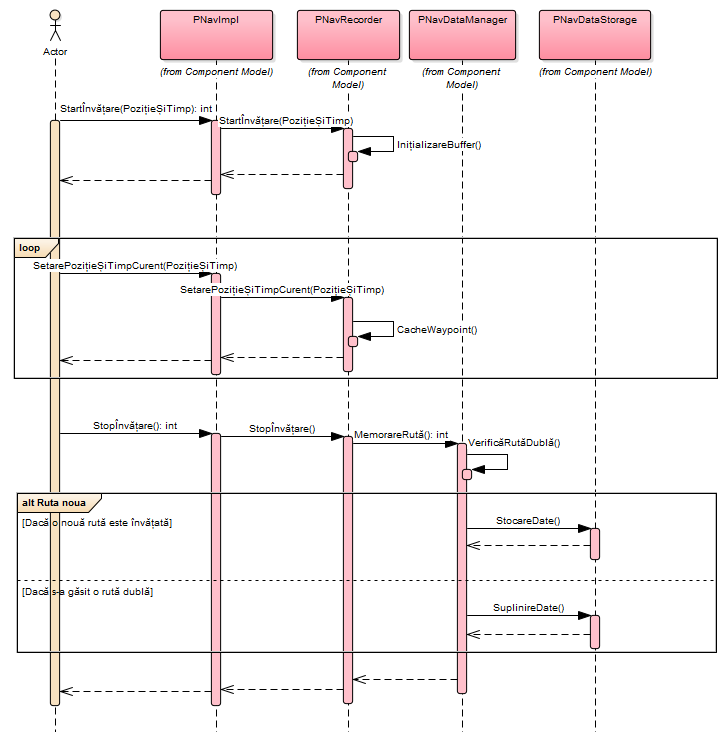
\includegraphics[width=0.9\textwidth]{Figures/rute_duble_sinc.png}}
   \caption{Procesul de verificarea al rutelor duble (sincron)}
   \end{figure}	
	
	În cazul în care ruta curentă are o secţiune similară cu o rută deja învăţată, unitatea software PNavDataManager va detecta secţiune respectivă şi va stoca numai waypoint-urile situate după aceasta. În schimb, toate destinaţiile sunt memorate. Criteriile pentru a detecta o astfel de rută sunt:
	
		\begin{enumerate}
	 \setlength\itemsep{0em}
		\item Destinaţia noii rute trebuie să fie situată într-o rază de 1km faţă de locaţia vechii destinaţii
		\item Punctul de start al noii rute trebuie să fie situată într-o rază de 1km faţă de punctul de plecare vechii destinaţii
		\item Toate waypoint-urile noii rute trebuie:
				\begin{enumerate}
				 \setlength\itemsep{0em}
					\item Să fie situat într-o anumită rază faţă de punctul de start al vechii rute
					\item Sau să fie situat într-o anumită rază faţă de destinaţia vechii rute
					\item Sau să fie situat într-o anumită rază faţă de un waypoint al vechii rute
				\end{enumerate}
	\end{enumerate}

Pragurile pot fi configurate înaintea procesului de compilare.


	\subsection{Filtrarea rutelor inutile}
	În timpul învăţării, rutele prea scurte (< 2km) nu vor fi stocate deoarece acest lucru ar însemna faptul că utilizatorul este destul de aproape de destinaţie.
	\vspace{6pt}
  \\Totodată, rutele foarte lungi (> 200km) vor fi de asemenea exclude din stocare deoarece ele nu reprezintă rute uzuale.
	\vspace{6pt}
  \\Pragurile pot fi configurate înaintea procesului de compilare.

\clearpage 

\section{Furnizarea predicţiilor} 
Pentru ca predicţiile să fie disponibile sunt necesari doi paşi.
\vspace{6pt}
\\Primul pas reprezintă încărcarea datelor relevante, în timp de al doilea constă în prioritizarea lor.

	\begin{figure}[h!]
   \centering
    \centering{%
      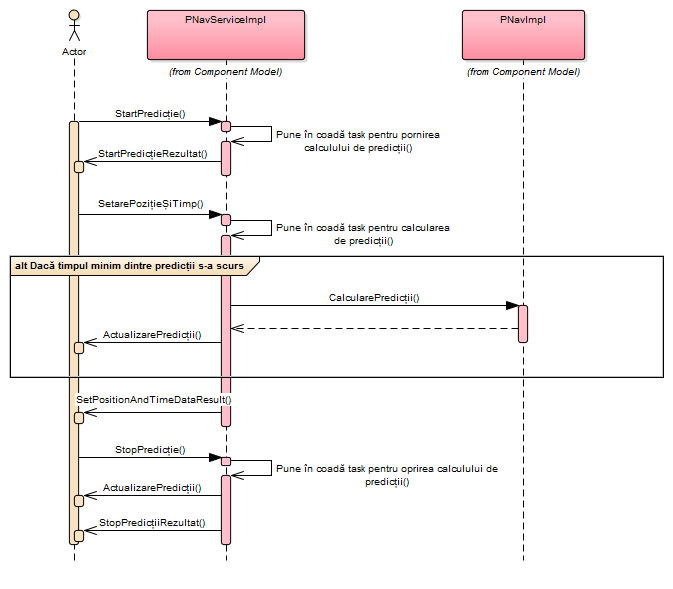
\includegraphics[width=0.9\textwidth]{Figures/calculare_predictii_asinc.png}}
   \caption{Procesul de calculare al predicțiilor(asincron)}
   \end{figure}	

	\subsection{Filtrarea datelor}
	Pentru o încărcare selectivă şi mai rapidă a datelor din unitatea PNavDataStorage, sunt create interogări. Sunt definiţi trei paşi în filtrare, unde pasul următor se excută doar în cazul în care cel curent nu a returnat destule rezultate:
		\begin{enumerate}
				 \setlength\itemsep{0em}
					\item Filtrarea rutei în funcţie de distanţa de la poziţia curentă la waypoint-urile rutelor
					\item Filtrarea rutei în funcţie de distanţa de la poziţia curentă la punctele de start ale rutelor
					\item Filtrarea rutelor în funcţie de timpul scurs până la ajungerea la destinaţie
		\end{enumerate}

	Toate rutele ce duc la o destinaţie situată la o distanţă mai mică de 1km faţă de poziţia actuală sunt ignorate deoarece utilizatorul aproape a ajuns la eventuala destinaţie.
	\vspace{6pt}
	\\În cazul predicţiilor baza pe timp, modulul furnizează o predicţie fără a cunoaşte ruta, ci doar destinaţia sa. Un astfel de caz ar fi cel în care utilizatorul a condus pe o rută în intervalul luni-miercuri, însă in ziua de joi a pornit de la o altă locaţie. Astfel, bazat pe timp, modulul prezice destinaţia fără a şti ruta corespunzătoare acesteia.
	
	
		\subsection{Frecvenţa predicţiei de rute}
		De obicei, waypoint-urile furnizate de modul de predicţie sunt transformate într-o rută ce foloseşte drumuri din hartă, fapt ce durează câteva secunde.
		Pentru a nu supraîncărca sistemul de navigaţie cu prea multe predicţii, dezvoltatorul poate seta timpul minim dintre două predicţii. Acestă setare se poate efectua chiar în timpul rulării.
		
		\subsection{Numărul maxim de predicţii}
		Pentru a putea suporta multiple platforme, modulul permite setarea numărului maxim de rute prezise ce apar deodată. Acestă setare se poate efectua chiar în timpul rulării.
		
		\subsection{Prioritizarea predicţiilor}
		Prioritatea unei rute reprezintă de fapt de probabilitatea ca această rută să fie ce pe care utilizatorul ar fi ales-o în mod uzual. Aceasta este exprimată sub formă de procente și se încadrează în intervalul 0\%-100\%.
		\vspace{6pt}
		\\Există mai multe criterii pentru a stabili prioritatea unei rute, fiecare dintre acestea fiind raportat la intervalul 0 (minimul) - 100 (maximul).  
		\vspace{6pt}
	    \\Pentru calcularea probabilității unei rute sunt necesari trei pași: 
	    
	    \begin{enumerate}
	     \setlength\itemsep{0em}
		 \item Pentru fiecare criteriu, se înmulțește ponderea cu probabilitatea sa 
		 \begin{equation}\label{qoat1}
		  SC = \sum_{i=1}^{n} p_{i}*c_{i}
		 \end{equation}
	     \item Se însumează toate criteriile  
		  \begin{equation}\label{qoat2}	      
	       SP = \sum_{i=1}^{n} p_{i}
	      \end{equation}
	     \item În urma raportului dintre suma de la pasul 1 și suma de la pasul 2, se obține probabilitatea rutei
	    \begin{equation}\label{qoat}	   
	     P = \frac{SC}{SP}
	    \end{equation}
    	\end{enumerate}
    	
		unde, \textit{P} = probabilitatea rutei, \textit{SC} = suma criteriilor, \textit{SP} = suma ponderilor, \textit{p} = ponderea criteriului, \textit{c} = probabilitatea criteriului (0\%-100\%), \textit{n} = numărul total de criterii	
		
		\vspace{6pt}
	    Metoda de definire a fiecărui criteriu depinde de criteriile însăși, după cum se observă în tabelele următoare.
		
		\begin{table}[!h]
		\caption{Criterii de prioritizare pentru predicţia bazată pe rute}
		\centering
		\begin{tabular}{ | m{2,7cm} | m{3,6cm} | m{3,22cm} | m{3,22cm} | m{1,4cm} | }
		\hline
		\textbf{Criteriu} & \textbf{Descriere} & \textbf{Min (0\% probabilitate)} & \textbf{Max (100\% probabilitate)} & \textbf{Pondere} \\ 
		\hline
		 Frecvenţa rutei & Numărul de utilizări al unei rute & Niciodată & Folosită de mai mult de 10 ori & 4 \\
		\hline
		 Frecvenţa rutei într-un anumit interval de timp & Numărul de utilizări al unei rute într-un anumit interval de timp (de la -1 oră la +2 ore) faţă de ora curentă & Niciodată & Folosită de mai mult de 10 ori & 1 \\
		\hline
		 Frecvenţa rutei într-o anumită zi & Numărul de utilizări al unei rute în ziua curentă din săptămână & Niciodată & Folosită de mai mult de 10 ori & 1 \\
		\hline
		 Frecvenţa rutei într-un anumit grup de zile & Numărul de utilizări al unei rute într-un anumit grup de zile (e.g. luni-vineri)& Niciodată &  Folosită de mai mult de 10 ori  & 1 \\
		\hline
		 Ultima utilizare a unei rute & Diferenţa dintre ultima utilizare a rutei şi ora/data curentă & >4 săptămâni & <2zile & 3 \\
		\hline
		 Distanţa până la destinaţie & Distanţa dintre poziţia actuală şi destinaţie & >100km & 0km & 1 \\
		\hline
		\end{tabular}
		\label{table:tabel_predictii}
		\end{table}
		
		
		\subsection{Predicţii bazate pe filtrarea rutei în funcţie de distanţa de la poziţia curentă la waypoint-urile rutelor}
		Criteriile definite în tabela ~\ref{table:tabel_predictii}, ``Criterii de prioritizare pentru predicţia bazată pe rute'' sunt extinse prin adăugarea următoarelor criterii:
		
		\begin{table}[!h]
		\caption{Criterii de prioritizare pentru predicţia bazată pe rutele din jurul unei poziţii}
		\centering
		\begin{tabular}{ | m{2,7cm} | m{3,6cm} | m{3,22cm} | m{3,22cm} | m{1,4cm} | }
		\hline
		\textbf{Criteriu} & \textbf{Descriere} & \textbf{Min (0\% probabilitate)} & \textbf{Max (100\% probabilitate)} & \textbf{Pondere} \\ 
		\hline
		 Distanţa până la rută & Distanţa dintre poziţia actuală şi waypoint-urile rutei &> 1km & 0km & 1 \\
		\hline
		 Direcţia către rută & Diferenţa dintre orientarea waypoint-urilor şi direcţia de navigare & 180$^{\circ}$ & 0$^{\circ}$ & 1 \\
		\hline
		\end{tabular}
		\end{table}
		
		
		\subsection{Predicţii bazate pe filtrarea rutei în funcţie de distanţa de la poziţia curentă la punctele de start ale rutelor}
		Criteriile definite în tabela ~\ref{table:tabel_predictii}, ``Criterii de prioritizare pentru predicţia bazată pe rute'' sunt extinse prin adăugarea următoarelor criterii:
		
		\begin{table}[!h]
		\caption{Criterii de prioritizare pentru predicţia bazată pe filtrarea rutele în funcţie de distanţa până la punctul de start al rutei}
		\centering
		\begin{tabular}{ | m{2,7cm} | m{3,6cm} | m{3,22cm} | m{3,22cm} | m{1,4cm} | }
		\hline
		\textbf{Criteriu} & \textbf{Descriere} & \textbf{Min (0\% probabilitate)} & \textbf{Max (100\% probabilitate)} & \textbf{Pondere} \\ 
		\hline
		 Distanţa până la punctul de start al rutei & Distanţa până la cel mai apropiat punct de start al rutei &> 3km & 0km & 1 \\
		\hline
		\end{tabular}
		\end{table}
		
		\subsection{Predicţii bazate pe filtrarea rutei în funcţie de timpul scurs până la ajungerea la destinaţie}
		Pentru acest caz sunt folosite criteriile definite în tabela ~\ref{table:tabel_predictii}, ``Criterii de prioritizare pentru predicţia bazată pe rute''.
		
	
\section{Eliberarea de spaţiu}   
Dacă pragul setat iniţial pentru dimensiunea maximă a bazei de date este atins, se va activa funcţia de eliberare a spaţiului. Aceasta va şterge obiectele cele mai vechi pentru a crea loc pentru obiectele noi.

	\begin{figure}[h!]
   \centering
    \centering{%
      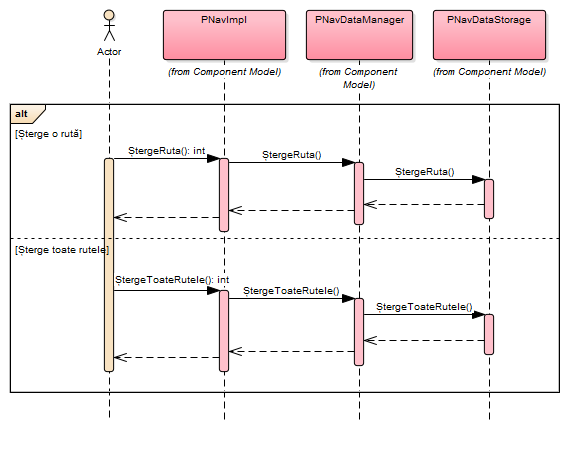
\includegraphics[width=0.7\textwidth]{Figures/sterge_ruta_sinc.png}}
   \caption{Procesul de ștergere a uneia sau mai multor rute (sincron)}
   \end{figure}	

		
		
		
		


	